\documentclass{beamer}
\usetheme{Madrid}
\usecolortheme{beaver}
\usepackage{amsmath}
\usepackage{verbatim}

\title{Conditional Neural Processes (ICML 2018)}
\subtitle{Marta Garnelo, Dan Rosenbaum, Chris J. Maddison, Tiago Ramalho, David Saxton, Murray Shanahan,
Yee Whye Teh, Danilo J. Rezende, S. M. Ali Eslami \\
DeepMind London }
\author{Tarandeep Singh}
\institute{IIT Hyderabad}
\date{\today}

\begin{document}

\begin{frame}
\titlepage
\end{frame}
\begin{comment}

\end{comment}
\section{Introduction}

\begin{frame}
\frametitle{Introduction}
\begin{itemize}
\item In deep supervised learning, given a dataset ${\{(x_i,y_i)\}}_{i=0}^{n-1}$ of n inputs where inputs $x_i\in X$ and outputs $y_i\in Y$, where there is an unknown function $f : X \rightarrow Y$, our algorithm returns an approximation function $g : X \rightarrow Y$, by minimizing loss b/w f and g.
\item Generally, this g is randomly initialized with a limited information about distribution of f. Due to this, deep neural networks spends most of the time learning specific task and fails to share learning with different task.
\begin{align}
    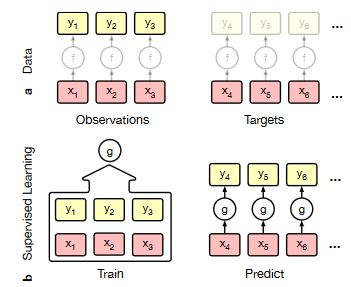
\includegraphics[scale=0.5]{supervised.JPG}
\end{align}
\end{itemize}
\end{frame}

\begin{frame}
\frametitle{Introduction}
\begin{itemize}
\item In Bayesian learning methods, prior information about distribution of f is used based on the practitioner's knowledge about f.
\item Bayesian inference is then based on conditioned functional space.
\item But Bayesian learning methods, become computationally expensive as dimensionality of dataset increases. Moreover, it is sometimes hard to design models from prior information.
\item If n is number of observations and m is number of targets, then complexity of these algorithms is $O((n+m)^3)$
\end{itemize}
  

\end{frame}
\begin{frame}
\frametitle{Conditional Neural Processes}

\begin{itemize}
\item In this paper, authors have proposed a new learning method that combines the function approximation power of supervised learning algorithms with knowledge and prior information about distribution.
\item The new family of models called \textit{Conditional Neural Processes(CNPs)}, proposed by authors define conditional distributions over functions given a set of observations.
\item CNPs are permutation invarient of observations O and $T\subseteq X$
\end{itemize}

\end{frame}

\begin{frame}
\frametitle{Conditional Neural Processes}
\begin{itemize}
\item The complexity of these algorithms is $O(n+m)$ making m predictions with n observations.
\end{itemize}
\begin{align}
    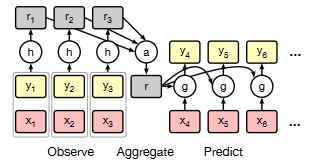
\includegraphics[scale=0.7]{cnps.JPG}
\end{align}
\end{frame}
\begin{frame}
\frametitle{Experimental Results of CNPs}
\begin{itemize}
\item \textbf{Pixel wise image regression }: Authors experimented with different number of context points(prior information or informed observations). They provided trained model with 1, 40, 200 and 728 context points and query the entire image.
\end{itemize}
\begin{align}
    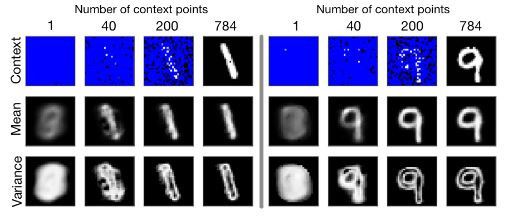
\includegraphics[scale=0.7]{pixelwise_Reg.JPG}
\end{align}
\end{frame}
\begin{frame}
\frametitle{Experimental Results of CNPs}
\begin{itemize}
\item \textbf{Pixel wise image generation}: Authors experimented with different number of context points. They provide the model with 1, 10, 100 and 1000 context
points and query the entire image.
\end{itemize}
\begin{align}
    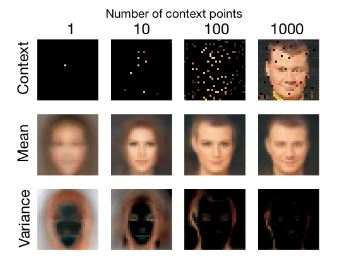
\includegraphics[scale=0.7]{pixelwise_gen.JPG}
\end{align}
\end{frame}

\begin{frame}
\frametitle{References}
\begin{itemize}
\item Marta Garnelo, Dan Rosenbaum, Christopher Maddison, Tiago Ramalho, David Saxton, Murray Shanahan, Yee Whye Teh, Danilo Jimenez Rezende, and S. M. Ali Eslami. Conditional neural processes. In Jennifer G. Dy and Andreas Krause, editors, Proceedings of the 35th International Conference on Machine Learning, ICML 2018, Stockholmsmässan, Stockholm, Sweden, July 10-15, 2018, volume 80 of Proceedings of Machine Learning Research, 1690–1699. PMLR, 2018. URL: http://proceedings.mlr.press/v80/garnelo18a.html.
\item \textbf{Code:} https://github.com/deepmind/neural-processes
\end{itemize}
\end{frame}

\end{document}
